\documentclass[a4paper]{article}
\usepackage{graphicx}
\usepackage{listings}
\usepackage[utf8]{inputenc}
\usepackage{caption}

\title{Trabajo Práctico\\``Transforma de Laplace\\y ecuaciones diferenciales''}
\author{Araneda, Alejandro – eloscurodeefeso@hotmail.com}
\date{1er. Cuatrimestre 2020\\Jueves, 2 de Julio}

\def\teacher{Juan Carlos Muñoz
\and Fabrizio Nocetti}

\captionsetup{justification=centering,labelsep=period,font={small},%
labelfont=bf,textfont=it}
\renewcommand{\tablename}{Tabla}
\renewcommand{\figurename}{Figura}
\renewcommand{\abstractname}{Resumen}
\renewcommand{\refname}{Referencias}
\let\originalcite\cite
\renewcommand{\cite}[2][]{\textsuperscript{\originalcite{#2}}}
% Cambiamos el estilo de las citas bibliograficas
\makeatletter\let\@afterindentfalse\@afterindenttrue\makeatother
% Para indentar primer parrafo
\setcounter{secnumdepth}{0}
% No se numeran las secciones pero si estan en el TOC 

\begin{document}

\begin{titlepage}\renewcommand\and\par\centering\makeatletter
    
\includegraphics{logo.png}\par
    {\Large Ingeniería en Computación \par}\vspace{0.5cm}
    {\LARGE Matemáticas Especiales \par}\vfill
    {\huge \@title \par}\vfill
    Alumno:\par
    \@author\vfill
    Práctica entregada:\par
    \@date\vfill
    Docentes:\par
    \teacher\vspace{1cm}\makeatother
\end{titlepage}

\begin{abstract}

    En el presente trabajo ejemplificamos el uso de la transformada
    de Laplace en la resolución de ecuaciones diferencias 
    construyendo una aplicación interactiva.

\end{abstract}

\section{Introducción}

\subsection*{Ecuaciones diferenciales}

Formalmente, una ecuación diferencial es aquella que en su 
expresión mate-mática pone en relación a una función y sus 
derivadas\cite{bib:zill}. Nuestro estudio se centra en las de primer órden, es 
decir, con presencia de hasta la primer derivada. 
De entre todas ellas tomamos las no homogéneas definidas 
sólo en coeficientes reales. De forma general:

\begin{equation}
    ay' + by + c = 0
    \label{eq:general}   
\end{equation}

Las ecuaciones diferenciales son una herramienta esencial en el 
diseño de modelos matemáticos de procesos reales, de uso común en
la ciencias de la física, química y otras. 

\begin{figure}[h]\centering
    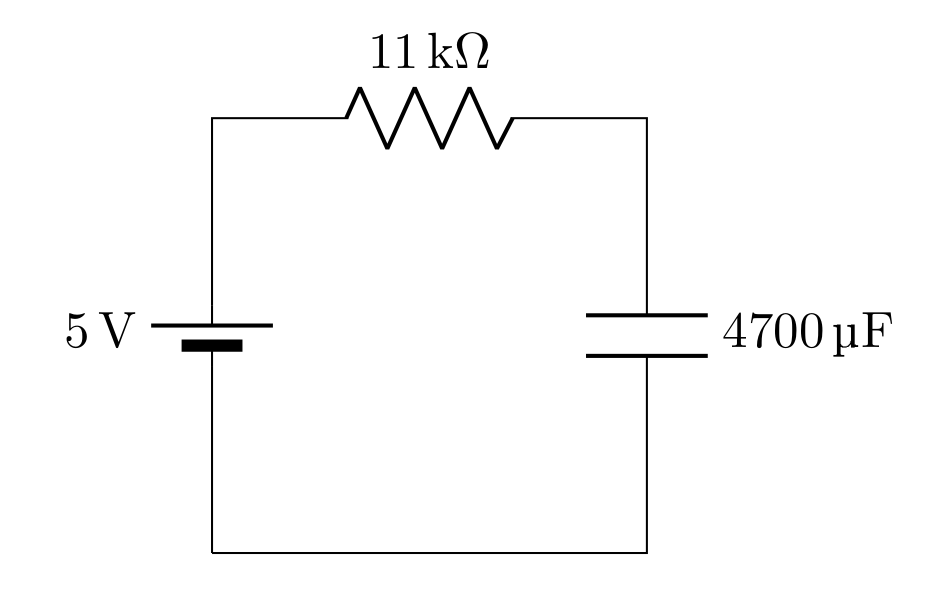
\includegraphics[height=4cm]{circuito.png}
    \caption{Ilustración de un circuito RC.}
    \label{fig:circuito}
\end{figure}

Por ejemplo, si analizamos el circuito RC (circuito con sólo 
resistores y capacitores) de la Figura \ref{fig:circuito} sometido 
a una tensión continua, aplicando las leyes de 
Kirchhoff y la definición de la corriente como diferencial de 
carga eléctrica en el tiempo, obtendremos:

\begin{equation}
    - R \cdot \frac{dq}{dt} - \frac{1}{C} \cdot q(t) + V = 0
    \label{eq:circuito}
\end{equation}

Donde $R$ es la resistencia en ohmios del resistor, $C$ es 
la capacitancia en faradios del capacitor, $V$ es la tensión
contínua de la fuente en voltios, y $q(t)$ es la carga en 
culombios del capacitor.

\subsection*{Transformada de Laplace}

La transformada de Laplace constituye un operador lineal sobre
funciones. Formalmente lo definimos con la siguiente integral 
impropia, siempre que exista:

\begin{equation}
    \mathcal{L}\left\{ f(t) \right\} 
    = \int_{0}^{\infty} e^{-st}f(t)dt=F(s)
\end{equation}

Nosotros en vez de la fórmula integral utilizamos tablas de
transformadas ya calculadas, como es el método habital. En la Tabla 
\ref{tab:laplace} se muestra un listado parcial de las mismas, 
conteniendo aquellas que son pertinentes para esta práctica.

{\renewcommand{\arraystretch}{2}
\begin{table}[h]\centering
    \begin{tabular}{|c|c|c|}
    \hline
    \# & $f(t)$      & $F(s)$                                         \\ \hline
    1  & $0$         & $0$                                            \\ \hline
    2  & $1$         & \scalebox{1.25}{$\frac{1}{s}$}                 \\ \hline
    3  & $t$         & \scalebox{1.25}{$\frac{1}{s^{2}}$}             \\ \hline
    4  & $f'(t)$     & $sF(s) - f(0)$                                 \\ \hline
    5  & $e^{-at}$   & \scalebox{1.25}{$\frac{1}{s+a}$} para $s>-a$   \\ \hline
    6  & $1-e^{-at}$ & \scalebox{1.25}{$\frac{a}{s(s+a)}$} para $s>0$ \\ \hline
    \end{tabular}
    \caption{Funciones y transformadas de Laplace}
    \label{tab:laplace}
\end{table}}

La utilidad de la transformada de Laplace en la resolución de 
ecuaciones diferenciales viene dada por varias de sus características:
al ser un operador lineal nos permite la factorización de 
coeficientes constantes; al tener inversa nos permiter obtener 
soluciones únicas; al operar con las transformadas se obtiene la
solución mediante procedimientos algebraicos. Si aplicamos la 
transformada a la Ecuación \ref{eq:general} obtenemos el siguiente 
desarrollo:

    \[ \mathcal{L}\left\{ ay' + by + c \right\} = \mathcal{L}\left\{ 0 \right\} \]
    \[ a \cdot \left[ s \mathcal{L}\left\{ y \right\} - y(0)\right] + b \cdot \mathcal{L}\left\{ y \right\} + c \cdot \frac{1}{s} = 0 \]

Despejando la ecuación para la transformada, y definiendo como
$d$ al valor de condición inicial $y(0)$, obtenedremos la
expresión más general de la que derivarán el resto de las
transformadas dependiendo del valor de los coeficientes:

\begin{equation}
    \mathcal{L}\left\{ y \right\} = \frac{ads - c}{s(as + b)}
\end{equation}

Para aplicar la antitransformada y obtener la función que
resuelve nuestra ecuación diferencial, debemos rescribir
la transformada mediante procedimientos algebraicos que 
permitan utilizar la tabla. Resolvemos el caso en el que
los coeficientes de la función y la derivada son distintos 
de cero:

    \[ \frac{ads - c}{s(as + b)} = \frac{ads - c}{as\left(s + \frac{b}{a}\right)} = d \cdot \frac{1}{\left(s + \frac{b}{a}\right)} - \frac{c}{b} \cdot \frac{\frac{b}{a}}{s\left(s + \frac{b}{a}\right)} \]
    \[ y = d \cdot \mathcal{L}^{-1}\left\{\frac{1}{\left(s + \frac{b}{a}\right)}\right\} - \frac{c}{b} \cdot \mathcal{L}^{-1}\left\{\frac{\frac{b}{a}}{s\left(s + \frac{b}{a}\right)}\right\} \]
    \[ y = de^{-\frac{b}{a}x} - \frac{c}{b}\left(1 - e^{-\frac{b}{a}x}\right) \]
\begin{equation}
    y = \left( d + \frac{c}{b} \right) e^{ - \frac{b}{a} x } - \frac{c}{b}  \label{eq:nonzero}
\end{equation}

Para verificar que la Ecuación \ref{eq:nonzero} es nuestra 
solución buscada, calculamos su derivada y remplazamos ambas 
expresiones en la Ecuación \ref{eq:general}, teniendo en 
cuenta que asumimos que ningún coeficiente es igual a cero:

    \[ a \cdot \left[ \left( - \frac{db}{a} - \frac{c}{a} \right) e^{ - \frac{b}{a} x } \right] + b \cdot \left[ \left( d + \frac{c}{b} \right) e^{ - \frac{b}{a} x } - \frac{c}{b} \right] + c = 0 \]
    \[ - \left( db + c \right) e^{ - \frac{b}{a} x } + \left( db + c \right) e^{ - \frac{b}{a} x } - c + c = 0 \]

Con lo que queda demostrado que es solución de nuestra ecuación
diferencial para el caso de que los coeficientes de la derivada
y la función sean distintos de cero, sin importar el valor del
término independiente ya que no forma parte de las restricciones
del dominio.

\section{Descripción de la Práctica}

\subsection{Enunciado}

Realizar una aplicación interactiva que resuelva ecuaciones 
diferenciales de primer orden no homogénea en coeficientes 
reales utilizando la transformada de Laplace.
La aplicación debe suministrar tanto la expresión matemática
de la solución como el resultado numérico en un punto del
dominio. 

\subsection{Entorno de Desarrollo}

Programamos la aplicacion en el lenguaje C, adhiriendo a las 
características y sintaxis según las normas ANSI C89/ ISO C90. 
Presentamos tanto una copia del código fuente 
como un anexo con la documención interna detallada. Para la 
autodocumentación interna se usa el formato Doxygen\cite{bib:doxy}.

\subsection{Instrucciones de Compilación}

La compilación de la aplicación para la plataforma del
sistema operativo Windows se realiza con el compilador portado 
en base al GCC de GNU por el proyecto de entorno de desarrollo 
MinGW\cite{bib:mingw}. Ubicados en el directorio raíz del código 
fuente, la línea de comandos es:

\begin{center}\ttfamily 
    gcc -o laplace -lm laplace.c reader/reader.c \\
    expr/expr.c eval/eval.c eval/solver.c 
\end{center}

\subsection{Generación de la Documentación}

La aplicación está profusamente documentada de forma que 
es posible obte-ner información detallada tanto de la 
organización de archivos, las estructuras de datos definidas
y las funciones que determinan su uso. Para generarla desde 
la línea de comandos en el directorio raíz de la documentación
utilizamos:

\begin{center}\ttfamily 
    doxygen 
\end{center}

\subsection{Dependencias}

El ejecutable producido es posible utilizarlo de manera 
independiente cum-pliendo con todos los requerimientos del 
enunciado. Sin embargo, mayor aprove-chamiento es posible
si se lo integra con el paquete de aplicaciones para la 
generación de gráficas Plotutils, del que también existe
una versión para la plataforma Windows, la que se distribuye
con nuestro desarrollo. 

\begin{figure}[tbp]\centering
    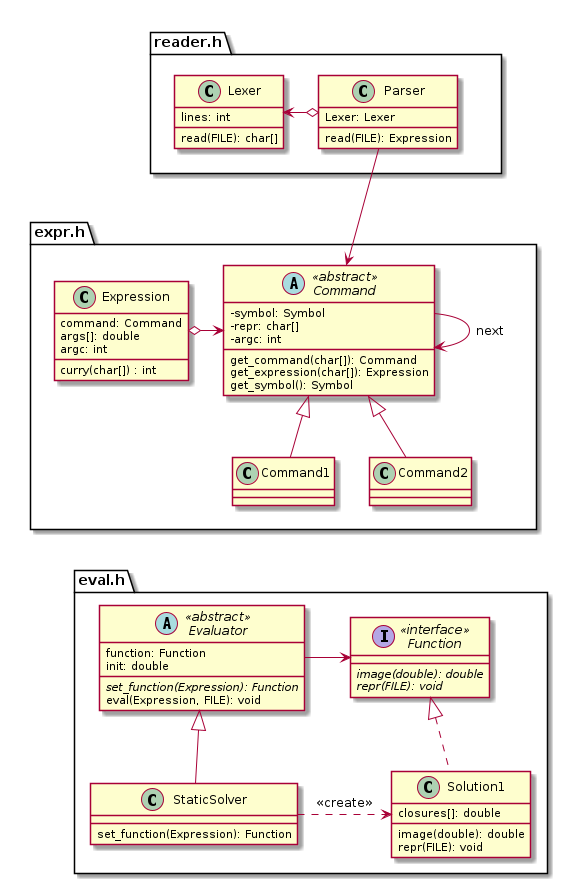
\includegraphics[height=.96\textheight]{laplace.png}
    \caption{Diagrama de clases en UML}
    \label{fig:class}
\end{figure}

\section{Diseño y Desarrollo}

Nuestra aplicación sigue el formato interactivo REPL (por las
siglas en inglés de \textit{Read, Eval, Print and Loop}) 
leyendo sus comandos de la terminal y volcando sobre la misma
su resultado en forma de conjunto de datos. 

Su utilización puede combinarse con la utilidad graficadora
{\ttfamily graph} de los sistemas tipo UNIX, implementada
en el paquete Plotutils de GNU\cite{bib:plot} y del que también existe 
versión portada para Windows\cite{bib:win}.

\subsection{Diagrama de Clases}

En la Figura \ref{fig:class} se puede observar el diagrama de
clases completo con todos los módulos de la aplicación, siguiendo
la normativa del lenguaje UML. 

\subsection{Patrones de Diseño}

La resolución de problemas frecuentes en el desarrollo de 
aplicaciones impone una fuerte necesidad de técnicas de diseño
que permitan la reutilización de código. Es así que en el
campo de la programación orientada a objetos surge el 
concepto de patrón de diseño \cite{bib:gof}.

\subsubsection{\textit{Forwarding} o Delegación}

El módulo {\ttfamily reader} encargado de hacer el análisis
sintáctico de los comandos ingresados sigue el patrón de 
Delegación o la técnica de \textit{Forwarding} (se distinguen
o emparentan por cuestiones técnicas según la bibliografía).

El analizador semántico correspondiente a la clase 
{\ttfamily Parser} delega la obtención de símbolos de la línea
de comando a la clase {\ttfamily Lexer} que hace las veces
de analizador lexicográfico.

\subsubsection{Cadena de responsabilidades}

El módulo {\ttfamily expr} complementa la tarea del analizador
semántico en la construcción del árbol de sintaxis abstracta
siguiendo el patrón de Cadena de responsabilidades.

Las instancias de la clase {\ttfamily Command} organizadas en
cadena, responden al {\ttfamily Parser} cuál de ellas es la 
responsable del comando que corresponde a la representación
que el analizador semántico ha identificado en el flujo de 
entrada.

\subsubsection{Método factoría}

El módulo {\ttfamily eval} es el responsable de modificar el
contexto de evaluación de acuerdo al árbol de sintaxis abstracta
que representa la clase {\ttfamily Expression}. Ya que utilizamos
clases concretas que implementan las distintas soluciones, la 
clase {\ttfamily Evaluator} se independiza del mecanismo de su 
creación mediante un método factoría.

La clase {\ttfamily StaticSolver} es la que implementa este 
método y selecciona cuál de la soluciones concretas creará,
las cuales a su vez deberán seguir la interfaz {\ttfamily Function}
para poder ser utilizadas por el evaluador.

\section{Análisis y Guía de Uso}

A continuación, luego de detallar la sintaxis de los comandos
reconocidos por nuestra aplicación, utilizamos un ejemplo concreto
para explicar su funcionamiento y realizar un análisis de los 
resultados obtenidos.

\subsection{Comandos reconocidos}

Ya sea a través de la línea de comandos o de un archivo encadenado
al flujo de entrada, nuestra aplicación recibe instrucciones que 
evalúa y con las que elabora resultados que a su vez pueden 
encadenarse con otras aplicaciones, como las generadoras de gráficos del 
paquete Plotutils. Son reconocidad las siguientes órdenes:

\begin{center}
\begin{tabular}{l p{.5\textwidth}}
    {\ttfamily init \textit{[value]}} & Establece el valor 
        inicial, correspondiente a $y(0)$. Por defecto es 0. \\
    {\ttfamily coef \textit{[indep [func [deriv]]]}} & Establece 
        los coeficientes de la ecuación diferencial. En orden: 
        término independiente, factor de la función y de su 
        derivada. Por defecto todos son 0.\\
    {\ttfamily repr} & Devuelve la expresión matemática de la 
        solución. No admite argumentos.\\
    {\ttfamily step \textit{[steps [gap [begin]]]}} & Genera 
        el conjunto de datos. Sus argumentos son: cantida de 
        puntos, distancia entre ellos, valor inial. Por 
        defecto son 20, 1 y 0.
\end{tabular}
\end{center}

\subsection{Caso de uso}

Para resolver la Ecuación \ref{eq:circuito} y obtener la
carga del capacitor en el tiempo correspondiente al 
circuito RC de la Figura \ref{fig:circuito} durante el 
régimen transitorio de carga, escribimos en un archivo 
de texto llamado {\ttfamily charge.edo} los siguientes 
comandos:

\begin{verbatim}
    init 0
    coef 5 -212.76 -11e3
    repr 
\end{verbatim}

Ejecutamos la aplicación redirigiendo el archivo 
{\ttfamily charge.edo} a su entrada con la siguiente
línea de commandos de la terminal:

\begin{center}\ttfamily
    laplace < charge.edo
\end{center}

Obtenemos como salida el siguiente texto:

\begin{verbatim}
    # y = -0.023501 * exp( -0.019342 * x ) + (0.023501)
\end{verbatim}

Con lo que comprobamos que en el momento incial o tiempo
cero, nuestro capacitor está descargado. A medida
que pasa el tiempo, se carga aproximándose exponencialmente
al valor de casi 24 miliculombios. Esta carga sobre la
capacitancia de 4700 microfaradios, nos indicaría que 
en ese momento casi toda la tensión de 5 voltios cae en el
componente. La constante de tiempo $\tau$ co-rresponde
al valor de $x$ que torna en $-1$ al exponente, lo que
coincide, como es de esperarse, con el producto de la
capacitancia por la resistencia de nuestro circuito.

\begin{figure}[htb]\centering
    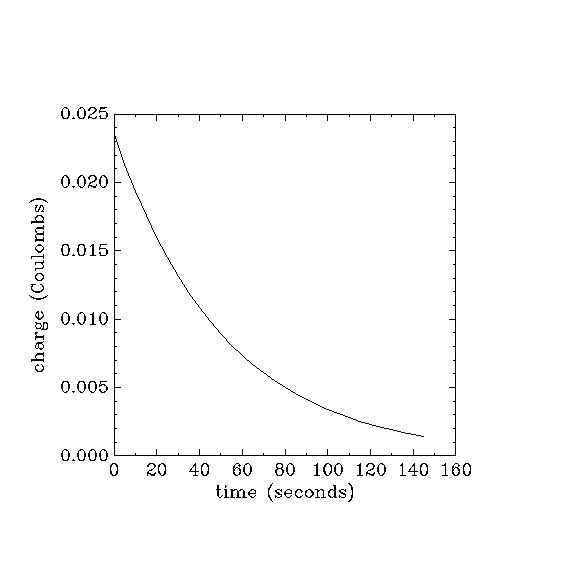
\includegraphics[height=9cm]{drain.png}
    \caption{Gráfica del conjunto de datos obtenidos con la aplicación}
    \label{fig:graph}
\end{figure}

Para analizar el régimen transitorio de descarga 
utilizamos otra caracterís-ticas de nuestra aplicación, 
escribiendo en un archivo de texto {\ttfamily 
drain.edo} los siguientes comandos:

\begin{verbatim}
    init 0.023501
    coef 0 -212.76 -11e3
    step 30 5 0
\end{verbatim}

Luego ejecutamos nuestra aplicación redirigiendo su
salida a otro archivo que llamamos {\ttfamily drain.dat}
 con la línea de comandos:

\begin{center}\ttfamily
    laplace < drain.edo > drain.dat
\end{center}

Finalmente, utilizamos este archivo con el conjunto
de datos para producir junto con 
la aplicación {\ttfamily graph} del paquete {\ttfamily 
plotutils} la Figura \ref{fig:graph} mediante la línea 
de comandos:

\begin{center}\ttfamily
    graph -T png -X "time (seconds)" \\ -Y "charge (Coulombs)" drain.edo > drain.png
\end{center}

\section{Conclusiones}

Si bien no nos hemos adentrado en el mundo de la ecuaciones
diferenciales más complejas donde la transformada de 
Laplace se torna realmente útil, hemos podido 
comprobar como reduce la tarea de hallar una solución 
empleando métodos algebraicos que de otra forma sino nos
obligaría a la integración y derivación.

Creemos que nuestra aplicación ha demostrado su utilidad
y que el diseño empleado es lo bastante flexible tanto
para ser integrado en una interfaz gráfica de usuario como
para extender fácilmente sus comandos y su alcance, por 
ejemplo, a ecuaciones de segundo grado.

Esta experiencia nos ha servido también para acercarnos a 
desarrollos orientados a la ciencia como son las utilidades
del paquete Plotutils, las que son integradas o 
reimplementadas por un buen número de aplicaciones 
comerciales.

\noindent\rule{\textwidth}{1pt}

\begin{thebibliography}{9}

\bibitem{bib:gof}
Gamma, E., \& Al, E. (2016). 
\textit{``Design patterns : elements of reusable object-oriented 
software''}. Boston: Addison-Wesley.

\bibitem{bib:zill}
Zill, D. G., M En C Andrés Sestier, Virgilio González Pozo, \& Al, E. (2000).
\textit{Ecuaciones diferenciales con aplicaciones de modelado}.
International Thomson Editores.

\bibitem{bib:mingw}
\textit{``MinGW.org GCC''}. 
(Version 9.2.0; MinGW.org Proyect: 2020).
Recuperado de http://www.mingw.org/

\bibitem{bib:doxy}
\textit{``Doxygen''}. 
(Version 1.8.19; Dimitri van Heesch.: 2018).
Recuperado de https://www.doxygen.nl/

\bibitem{bib:plot}
\textit{``GNU plotutils''}.
(Version 2.6; Free Software Fundation, Inc.: 2009).
Recuperado de https://www.gnu.org/software/plotutils/

\bibitem{bib:win}
\textit{``PlotUtils for Windows''}.
(Version 2.4.1; GnuWin Proyect: 2004).
Recuperado de http://gnuwin32.sourceforge.net/packages/plotutils.htm

\end{thebibliography}

\end{document}
